\documentclass{pgnotes}

\title{Space planning}

\begin{document}

\section{Form factor}

\section{Equipment layout}

IT equipment is mounted in racks within cabinets.
Cabinets make up rows and pairs of rows make up aisles.


\subsection{Cabinet}

A cabinet contains front-and-back vertical rack rails, and is secured by a lockable door, usually perforated.
Equipment is racked within the cabinet.
Standard full-size cabinets are 42U in height, with each position numbered from the bottom upwards.

\begin{figure*}[htbp]
  \centering
  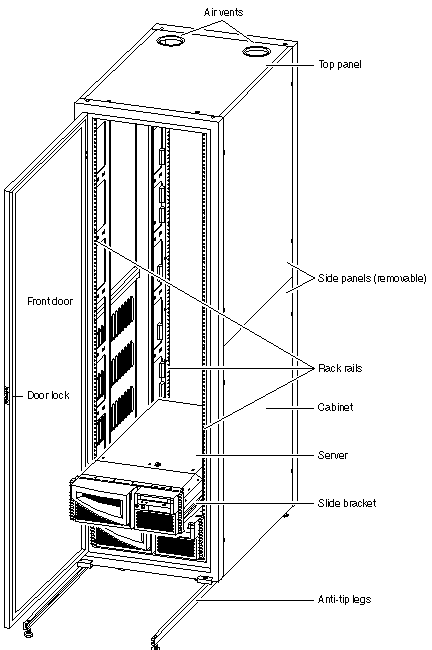
\includegraphics[width=1.0\linewidth,height=0.8\paperheight,keepaspectratio]{cabinet}
  \caption{19-inch cabinet schematic (Oracle)}
  \label{fig:cabinet}
\end{figure*}

Most servers, like desktop computers, are air cooled.
Air is drawn in at the front and ejected out the rear of the server.
Servers are always racked front-to-back.

\begin{figure}[htbp]
  \centering
  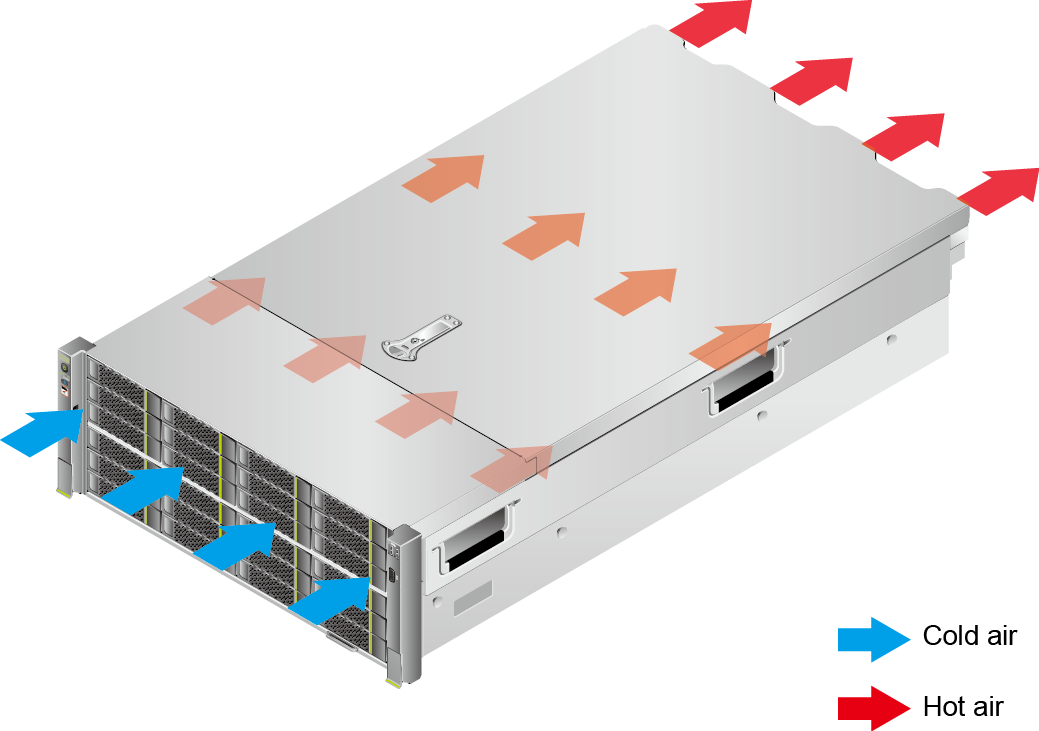
\includegraphics[width=0.5\linewidth]{server_airflow_huawei}
  \caption{Conventional front-to-back server airflow}
  \label{fig:server-airflow}
\end{figure}

Cabling is normally done at the rear of the rack.
Networking and power distribution equipment is often (but not always) mounted at the rear of a cabinet facing the rear.

\subsection{Rack mounting}

Racks have holes drilled in them for allowing equipment to be secured.
These are normally unthreaded, and allow cage nuts and bolts to be inserted.
The cage nut inserts into the rack, whilst the bolt is inserted through the holes drilled in the IT equipment's rack ears.

\begin{figure}[htbp]
  \centering
  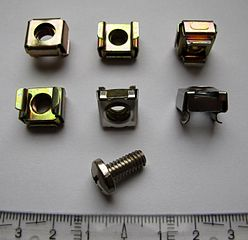
\includegraphics[width=0.75\linewidth]{cage_nut}
  \caption{Cage nuts and bolt (wikipedia)}
  \label{fig:cage-nut}
\end{figure}

Heavier pieces of equipment such as servers normally are placed on horizontal rails inserted into the rack first.
The rails are secured to the front and back racks.

\subsection{Rack units}

IT equipment in data centre environments is normally rack-mount form.
Rack-mount equipment has a standard width of \SI{48.3}{\centi\metre} or 19~inches, which includes the rack ears protruding from the side of each piece of equipment.

Equipment height is standardised in multiples of \SI{44.5}{\milli\metre} or 1.752~inches.
One rack unit (commonly called 1U) is equivalent to \SI{44.5}{\milli\metre}.
Conventionally we just use the number of units, such as 4U.


\subsection{Non-rackmount equipment}

Non-rackmount equipment such as tower-type server PCs should be discouraged in data centre environments.
Sometimes legacy equipment has to be accomodated.

\section{Good practices}

\begin{enumerate}

\item Leave sufficient space surrounding racks to allow easy access to the front and the rear.

\item Sufficient space must be provided to allow easy insertion and removal of equipment.

\item Lighting must be adequate so that you can see front and back of the rack safely.

\end{enumerate}

\end{document}